\documentclass[10pt]{report}
\usepackage{csquotes}
\usepackage{titlesec}

\usepackage{fancyhdr} % Required for custom headers
\usepackage{lastpage} % Required to determine the last page for the footer
\usepackage{extramarks} % Required for headers and footers
\usepackage{graphicx} % Required to insert images
\usepackage{multirow}
\usepackage{array}
\usepackage{lipsum} % Used for inserting dummy 'Lorem ipsum' text into the template
\usepackage{epstopdf} % to include eps graphics pdf
\usepackage{listings}
\usepackage{color}
\usepackage{caption}
\usepackage[a4paper,total={6in, 4in}]{geometry}
\usepackage{graphicx}
\usepackage{fancyhdr}
\usepackage[a4]{crop}
\usepackage{tikz}
\usepackage{float}
\usepackage{amsmath}
\usepackage{setspace}
\usetikzlibrary{calc}
\usepackage{subfig}
\usepackage{titlesec}
\usepackage{pdfpages}
%\newcommand{\sectionbreak}{\clearpage}
\topmargin=-0.45in
\evensidemargin=0in
\oddsidemargin=0in
\textwidth=6.5in
\textheight=9.5in
\headsep=.50in 
\footskip=.50in

\usepackage{chngcntr}
\counterwithin{figure}{chapter}

\linespread{1.5}
% Line spacing
%\titleformat*{\section}{\LARGE\bfseries}
%\titleformat*{\subsection}{\Large\bfseries}
%\titleformat*{\subsubsection}{\Large\bfseries}
%\titleformat*{\paragraph}{\large\bfseries}
%\titleformat*{\subparagraph}{\large\bfseries}

% Set up the header and footer
\pagestyle{fancy}
%\nouppercase
\lhead{} % Top left header
\chead{} % Top center header
\rhead{\nouppercase{\leftmark}}  % Top right header
%{Real time pedestrian detection using CENTRIST feature with distance estimation
\lfoot{Dept of Electronics, Model Engineering College} % Bottom left footer
\cfoot{} % Bottom center footer
\rfoot{\thepage} % Bottom right footer
\renewcommand\headrulewidth{0.4pt} % Size of the header rule
\renewcommand\footrulewidth{0.4pt} % Size of the footer rule

\setlength\parindent{0pt} % Removes all indentation from paragraphs

%----------------------------------------------------------------------------------------
%	TITLE PAGE
%----------------------------------------------------------------------------------------
\tolerance=1
\emergencystretch=\maxdimen
\hyphenpenalty=10000
\hbadness=10000

\begin{document}




\begin{titlepage}
\pagestyle{empty}
\begin{tikzpicture}[overlay,remember picture]
\draw [line width=3pt,rounded corners=1pt,]
    ($ (current page.north west) + (1cm,-1cm) $)
    rectangle
    ($ (current page.south east) + (-1cm,1cm) $);       
\end{tikzpicture}
\newcommand{\HRule}{\rule{\linewidth}{0.5mm}} % Defines a new command for the horizontal lines, change thickness here

\center % Center everything on the page
 
%----------------------------------------------------------------------------------------
%	HEADING SECTIONS
%----------------------------------------------------------------------------------------
\linespread{1.0}
%% \HRule \\[0.1cm]
    {\Huge \bfseries WATCHDOG TIMER AND BROWNOUT DETECTOR FOR SAFETY CRITICAL APPLICATIONS


 \par}

\vspace{1.1cm}
   % \HRule \\[1.5cm]
%{ \huge \bfseries  REAL TIME PEDESTRIAN DETECTION USING CENTRIST FEATURE WITH DISTANCE MEASURE } \\[0.5cm] % Title of your Presentation
%\\[0.5cm]
\LARGE \bfseries PROJECT REPORT\\[1.25cm] % report name
\large \emph{Submitted to \\the APJ Abdul Kalam Technological University\\ 
 in partial fulfillment of the requirement for the award of
Degree of\\ Bachelor of Technology in Electronics and Communication Engineering}
\\[2cm] % Minor heading such as course title

%----------------------------------------------------------------------------------------
%	LOGO SECTION
%----------------------------------------------------------------------------------------


\includegraphics[scale=.75]{mec.png}\\ % Include a department/university logo - this will require the graphicx package
 

%----------------------------------------------------------------------------------------
%	AUTHOR SECTION
%----------------------------------------------------------------------------------------

% If you don't want a supervisor, uncomment the two lines below and remove the section above
\Large \emph{BY}\\

MENNY THANKACHAN (MDL17EC)\\
CHRISTINA ANN ZACHARIAH (MDL17EC)\\
REJOHN SLEEBA C (MDL17EC)\\
JEWEL JOSEPH (MDL17EC)\\[1cm]


%-------------------------------------------------------------------------------------------
\large \emph{Department of Electronics, \\
Model Engineering College, \\ Thrikkakara,
Kochi-682021,\\  Kerala.}
\\[0.5cm] % Minor heading such as course title

\Large \emph{JUNE 2021}
%----------------------------------------------------------------------------------------

\vfill % Fill the rest of the page with whitespace

\end{titlepage}


\newpage
\thispagestyle{empty}
\linespread{1.4}
\Large \begin{center} \textbf{DEPARTMENT OF ELECTRONICS}\\
\Large \textbf{MODEL ENGINEERING COLLEGE}\\
\large \textbf{THRIKKAKARA, KOCHI-682021}\\[0.5cm]

\includegraphics[scale=.5]{mec.png}\\
{ \Large \bfseries \underline {CERTIFICATE}} \\\end{center}  

This is to certify that this Seminar  entitled \emph{\textbf{FPGA BASED CONVOLUTIONAL NEURAL NETWORK ACCELERATOR FOR EMBEDDED APPLICATIONS}} is the  bonafide record of work carried out by  \textbf{MENNY THANKACHAN (MDL16EC), CHRISTINA ANN ZACHARIAH (MDL16EC007), REJOHN SLEEBA C (MDL16EC)} and \textbf{JEWEL JOSEPH (MDL16EC)} in partial fulfillment of the requirements for the completion of Degree of Bachelor of Technology in Electronics and Communication Engineering, at the Department of Electronics, Model Engineering College, Thrikkakara,Kochi.\\ 

{\bf Mr. Sajeesh M}  \hspace*{1cm} {\bf Mr. Irshad Ali T.K }\hspace*{3cm}{\bf Dr. Jayasree V.K. }\\



{\bf{Project Guide} \hspace*{0.5 cm}{\bf Project co-ordinator }\hspace*{0.3 cm}\hspace*{0.2cm}{\bf   Head of the Department}}\\
%\begin{center}Examiner (External) \end{center}



%----------------------------------------------------------------------------------------
%	TABLE OF CONTENTS
%----------------------------------------------------------------------------------------

\newpage
\linespread{1.5}
%\setcounter{tocdepth}{1} % Uncomment this line if you don't want subsections listed in the ToC
%\fontsize{12}{14}
\thispagestyle{empty}
 \begin{center}\huge \bfseries  {ACKNOWLEDGEMENT} \\[1.5cm]\end{center}  
 I express my sincere gratitude to  \textbf{Prof. (Dr.) Vinu Thomas}, Principal, Govt. Model Engineering College, Thrikakkara. I also thank  \textbf{Prof. (Dr.) Jayasree V.K.}, HOD of Electronics Engineering for providing us with the
college facilities we required for the completion of the project.
I express my heartfelt gratitude to  \textbf{Mr.Irshad Ali}, Assistant Professor,, Department of Electronics who has helped and motivated us.We are also thankful to our guide, \textbf{Mr Sajeesh M} Associate Professor in Department of Electronics Engineering, for his support and also the struggle she has made for planning the schedule
for our project.
On this occasion, we also remember the valuable suggestions and prayers oered by our family members, classmates and friends which were inevitable for the successful completion of the project
 \begin{raggedright}   \hspace{350pt}  \end{raggedright}

\vfill





\newpage


%\fontsize{12}{14}
\thispagestyle{empty}
 \begin{center}\huge \bfseries  {ABSTRACT} \\[1.5cm]\end{center}  
\par 
 


\newpage


\clearpage
%\setcounter{page}{1}
%----------------------------------------------------------------------------------------
%	TABLE OF CONTENTS
%----------------------------------------------------------------------------------------

%\setcounter{tocdepth}{1} % Uncomment this line if you don't want subsections listed in the ToC
\pagenumbering{roman}
%\fontsize{12}{14}
\newpage
\thispagestyle{empty}
 
\thispagestyle{empty}
\tableofcontents
%\newpage
\thispagestyle{empty}
 
\listoffigures
 
\listoftables
 \newpage

\clearpage
\pagenumbering{arabic}
\setcounter{page}{1}
\setstretch{1.3}
\chapter{Introduction}
 



\section{Motivation}



\section{Problem Statement and Objectives}
Boosted by an ever increasing high computational AI systems, AI chip architecture is presently one of the hottest researched fields, churning out processors architecture at a very rapid pace. All the major manufactures including Intel, Nvidea and AMD have been on the forefront of this innovation and this results in an architecture landscape that is changing everyday.  These architectures focus on different facets such as efficiency, memory management, computing power etc. Since a lot of these architectures are developed independently, there is a need to study about the different architecture styles and develop architectures by deriving from the the current styles by focussing on high performance and high efficiency.
The objectives are :
 \begin{enumerate}

 	\item Carry out a comparative study of the present architecture styles of AI processors.
 	\item Study and analyse a recently developed AI processor architecture that combines high performance with high efficiency.
 	\item Propose a new architecture that improves on the above mentioned architecture style.
 	  
 \end{enumerate}
   
\section{Major contribution of the Dissertation}
 
\begin{itemize}


\item The need for AI accelerators are introduced.
  
\item Two very popular and radically different AI architectures ( DaDianNao and EYERISS ) that focus both on efficiency and computation are studied in depth to derive motivation for new architectures.

\item A new AI processor architecture that improves on the state of the art architecture is studied in detail with focus on its communication aspect.

\end{itemize}
\section{Thesis Outline}

\newpage

\chapter{Literature Survey}

Your literature Survey

\newpage

\chapter{Proposed System}
Your proposed system
\newpage

\chapter{Implimentation}
implimentation of your project
\newpage

\chapter{Results and Analysis}

The following are the results of the project:
\begin{itemize}
    \item Individual modules of watchdog timer was designed in verilog and its functions were verified using testbench.
    \item Individual modules of burnout detector was designed in verilog and its functions were verified using testbench.
    \item Watchdog timer and burnout detector were integrated together in a top module with a common configuration register storing the values of constants.
    \item The functionality of the top module was verified using testbench.
    
\end{itemize}

\begin{figure}[h]
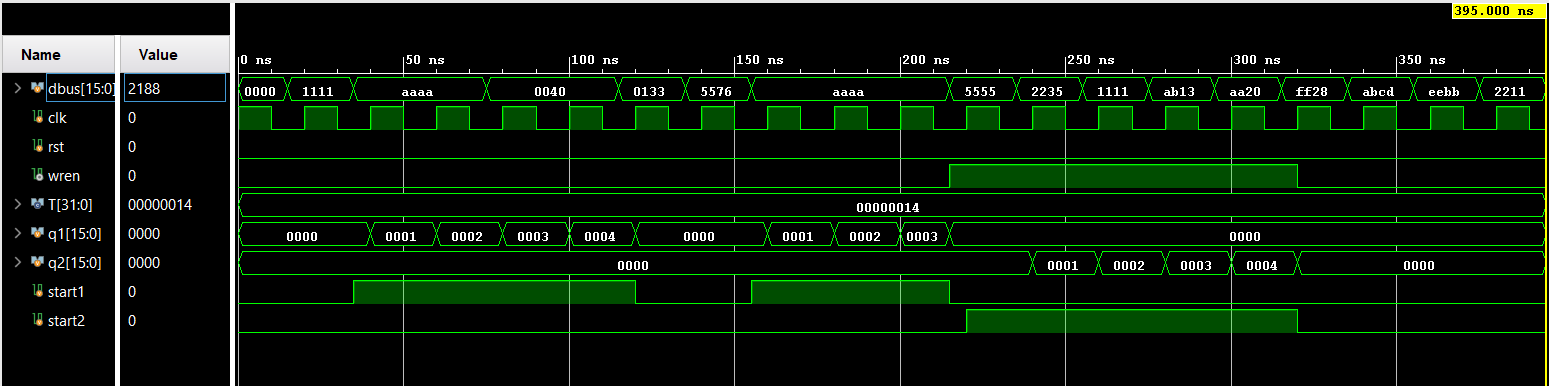
\includegraphics[width=\textwidth,height=\textwidth,keepaspectratio]{pattern_comparator.png}
\caption{Pattern comparator waveform}
\end{figure}

\begin{figure}[h]
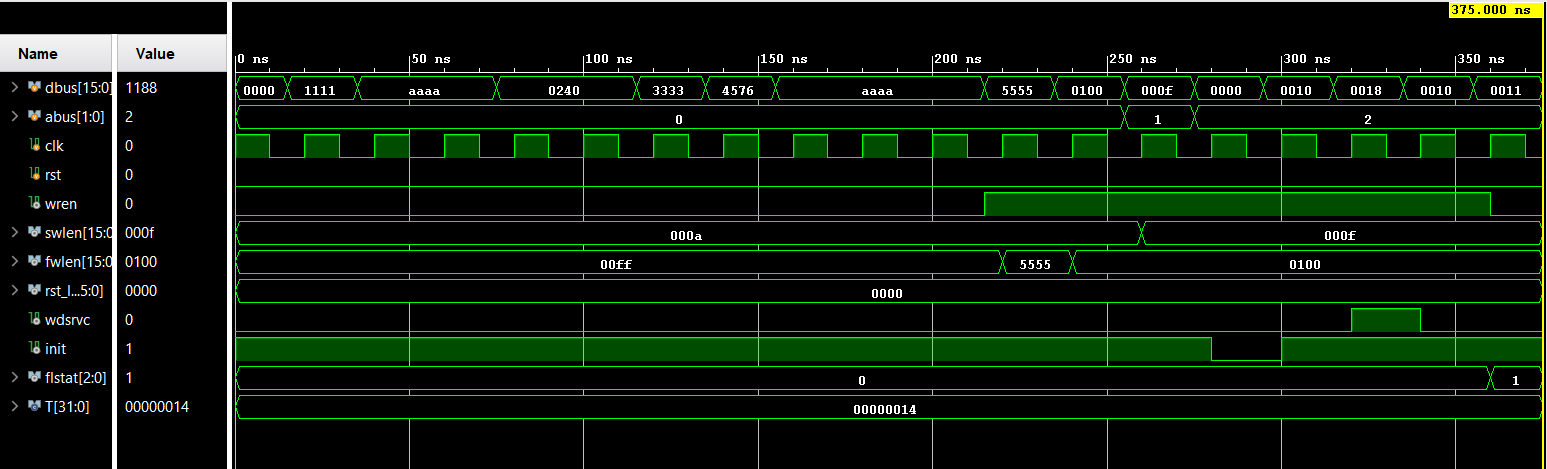
\includegraphics[width=\textwidth,height=\textwidth,keepaspectratio]{configuration_register.png}
\caption{configuration register waveform}
\end{figure}

\begin{figure}[h]
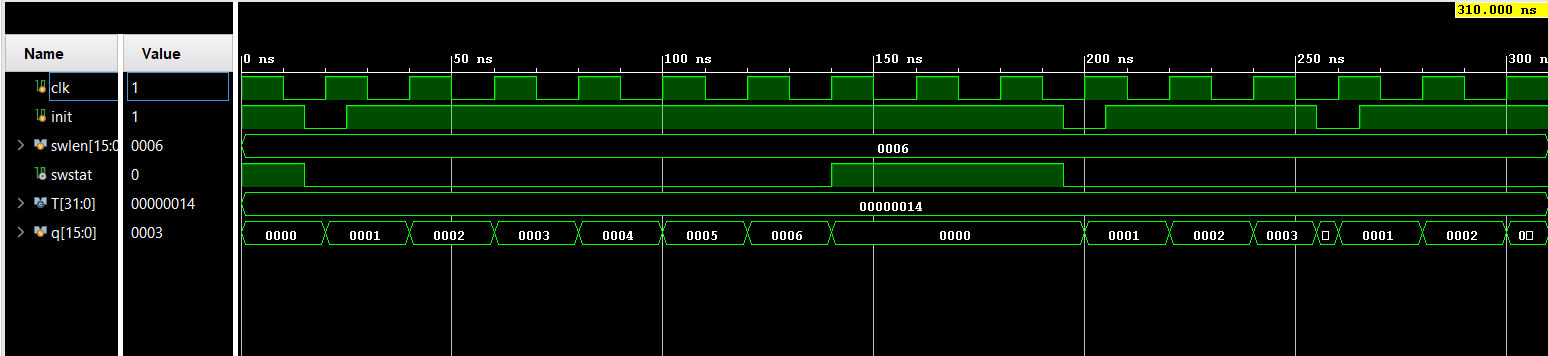
\includegraphics[width=\textwidth,height=\textwidth,keepaspectratio]{service_window.png}
\caption{service window waveform}
\end{figure}

\begin{figure}[h]
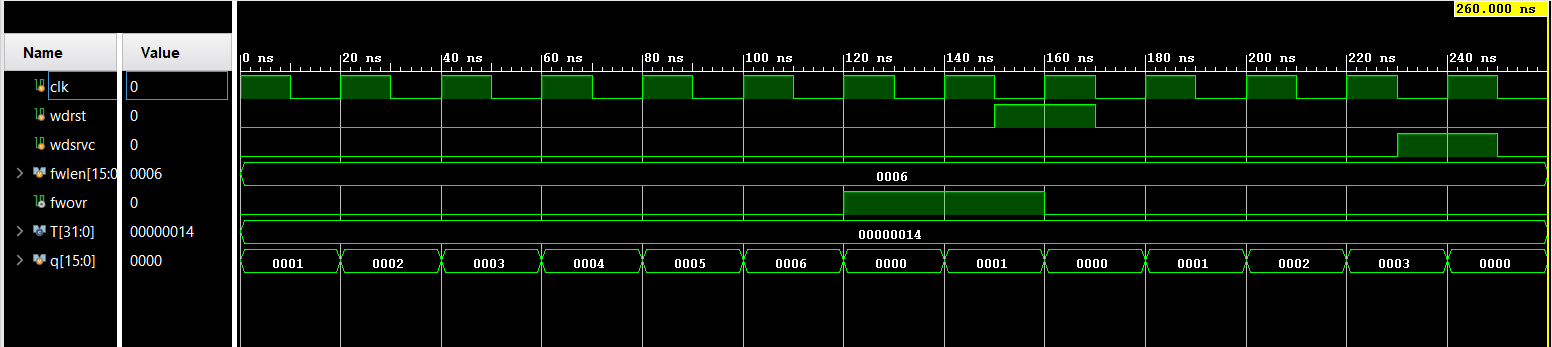
\includegraphics[width=\textwidth,height=\textwidth,keepaspectratio]{frame_window.png}
\caption{frame window waveform}
\end{figure}

\begin{figure}[h]
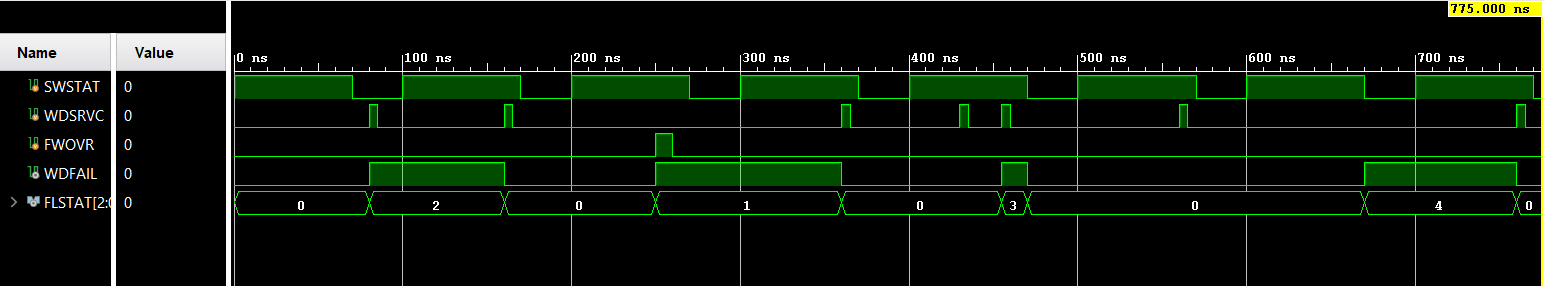
\includegraphics[width=\textwidth,height=\textwidth,keepaspectratio]{wd_fail_detector.png}
\caption{watchdog fail detector waveform}
\end{figure}

\begin{figure}[h]
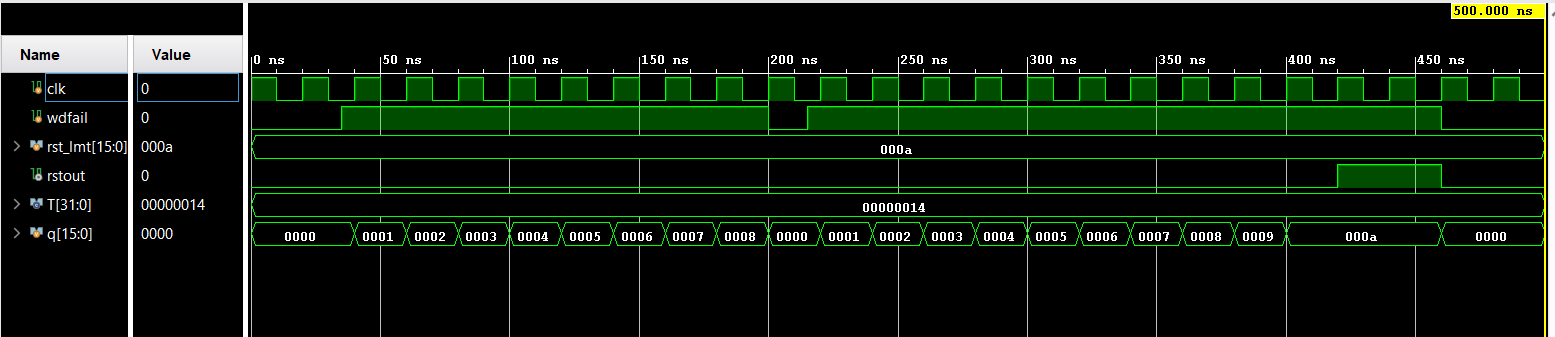
\includegraphics[width=\textwidth,height=\textwidth,keepaspectratio]{down_counter.png}
\caption{down counter waveform}
\end{figure}

\begin{figure}[h]
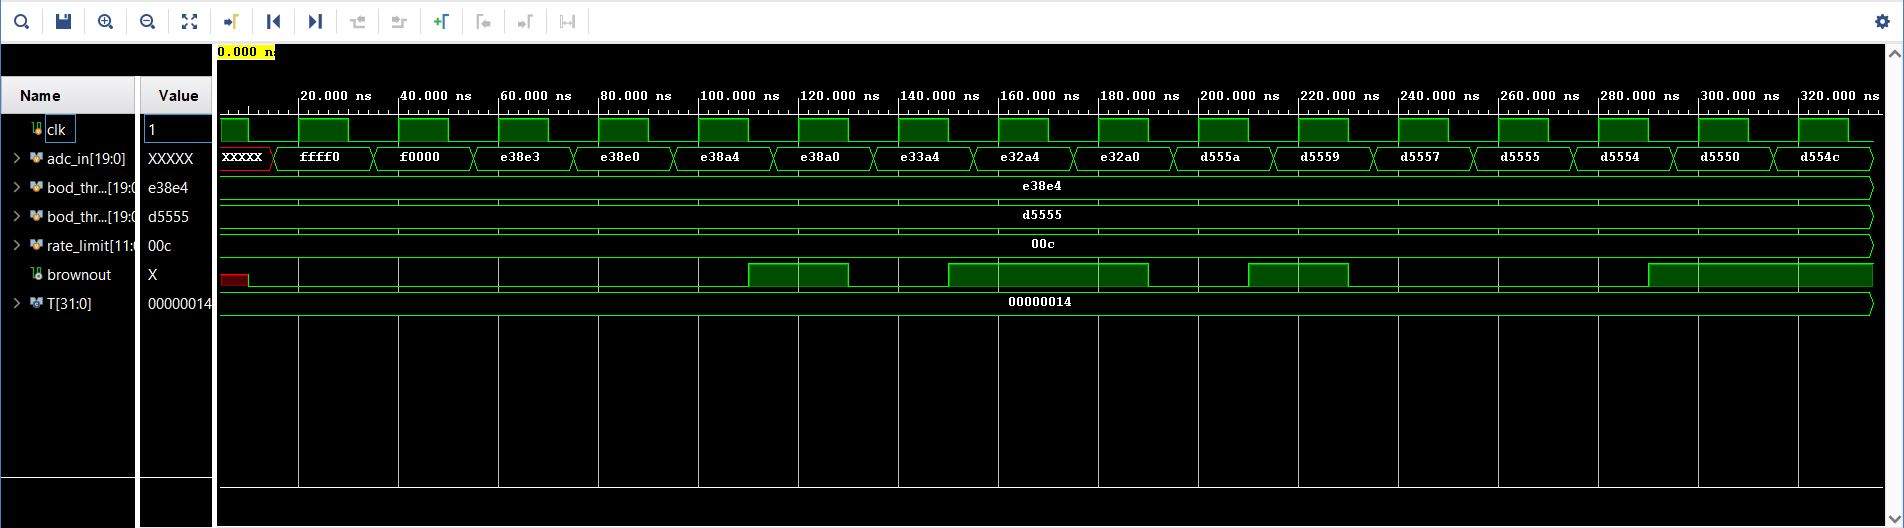
\includegraphics[width=\textwidth,height=\textwidth,keepaspectratio]{Brownout_output.JPG}
\caption{brownout detector waveform}
\end{figure}


\newpage
\chapter{Conclusion}
Your Conclusion 
\newpage
\begin{thebibliography}{999}
\addcontentsline{toc}{chapter}{REFERENCES}

\bibitem{} Watchdog timer IP core, Lattice Semiconductor, June 2020
\bibitem{} Unni, Ravi Krishnan, P. Vijayanand, and Y. Dilip. "FPGA Implementation of an Improved Watchdog Timer for Safety-critical Applications." 2018 31st International Conference on VLSI Design and 2018 17th International Conference on Embedded Systems (VLSID). IEEE, 2018.

\bibitem{} Straka, Bartholomew. "Implementing a microcontroller watchdog with a field-programmable gate array (FPGA)." (2013).
\bibitem{} Amer, Hassanein, and Ahmed Sobeih. "Increasing the Reliability of the Motorola MC68HC11 in the Presence of Temporary Failures." 11th IEEE Mediterranean Electrotechnical Conference (IEEE Cat. No. 02CH37379). IEEE, 2002.

\end{thebibliography}
\end{document}
